\documentclass{article}

% 页面边距设置
\usepackage[margin=1in]{geometry}

% 中文支持，fandol 是 TeX Live 自带中文字体，适合 Ubuntu
\usepackage[fontset=fandol]{ctex}

% 行距、示例文本、图片
\usepackage{setspace}
\usepackage{lipsum}
\usepackage{graphicx}
\graphicspath{{figures/}}

% 数学公式相关宏包
\usepackage{amsmath}
\usepackage{amssymb}
\usepackage{bm}

% 超链接，通常放在较后位置
\usepackage{hyperref}
\hypersetup{
	colorlinks = true,
	bookmarksopen = true,
	bookmarksnumbered = true,
	pdftitle = {VSCode and TeX Live Test File},
	pdfauthor = {Andy}
}

% 参考文献格式
\bibliographystyle{plain}

% 上标引用命令
\newcommand{\upcite}[1]{\textsuperscript{\cite{#1}}}

% 修改目录标题
\renewcommand{\contentsname}{\centerline{Contents}}

\title{\heiti\zihao{2} VSCode + TeX Live 测试文档}
\author{\songti Andy}
\date{2026年5月28日}

\begin{document}

\maketitle
\thispagestyle{empty}

\begin{abstract}
这是一个用于测试 Ubuntu + VSCode + TeX Live + LaTeX Workshop 配置的示例文件。
本文档主要用于检查中文显示、英文显示、图片插入、目录生成、公式编号、
交叉引用以及参考文献功能是否正常。
\end{abstract}

\tableofcontents

\section{Basic Text Test}

This is an English sentence for testing.

这是一句中文测试文本，用于确认 \LaTeX{} 是否能够正确支持中文显示。

这里还可以测试中英文混排，例如：VSCode, TeX Live, LaTeX Workshop 和 Ubuntu。

\section{Figure Test}

下面测试图片插入功能。如图~\ref{fig:example} 所示，图片文件应该放在当前目录下的 \verb|figures| 文件夹中。

\begin{figure}[htbp]
	\centering
	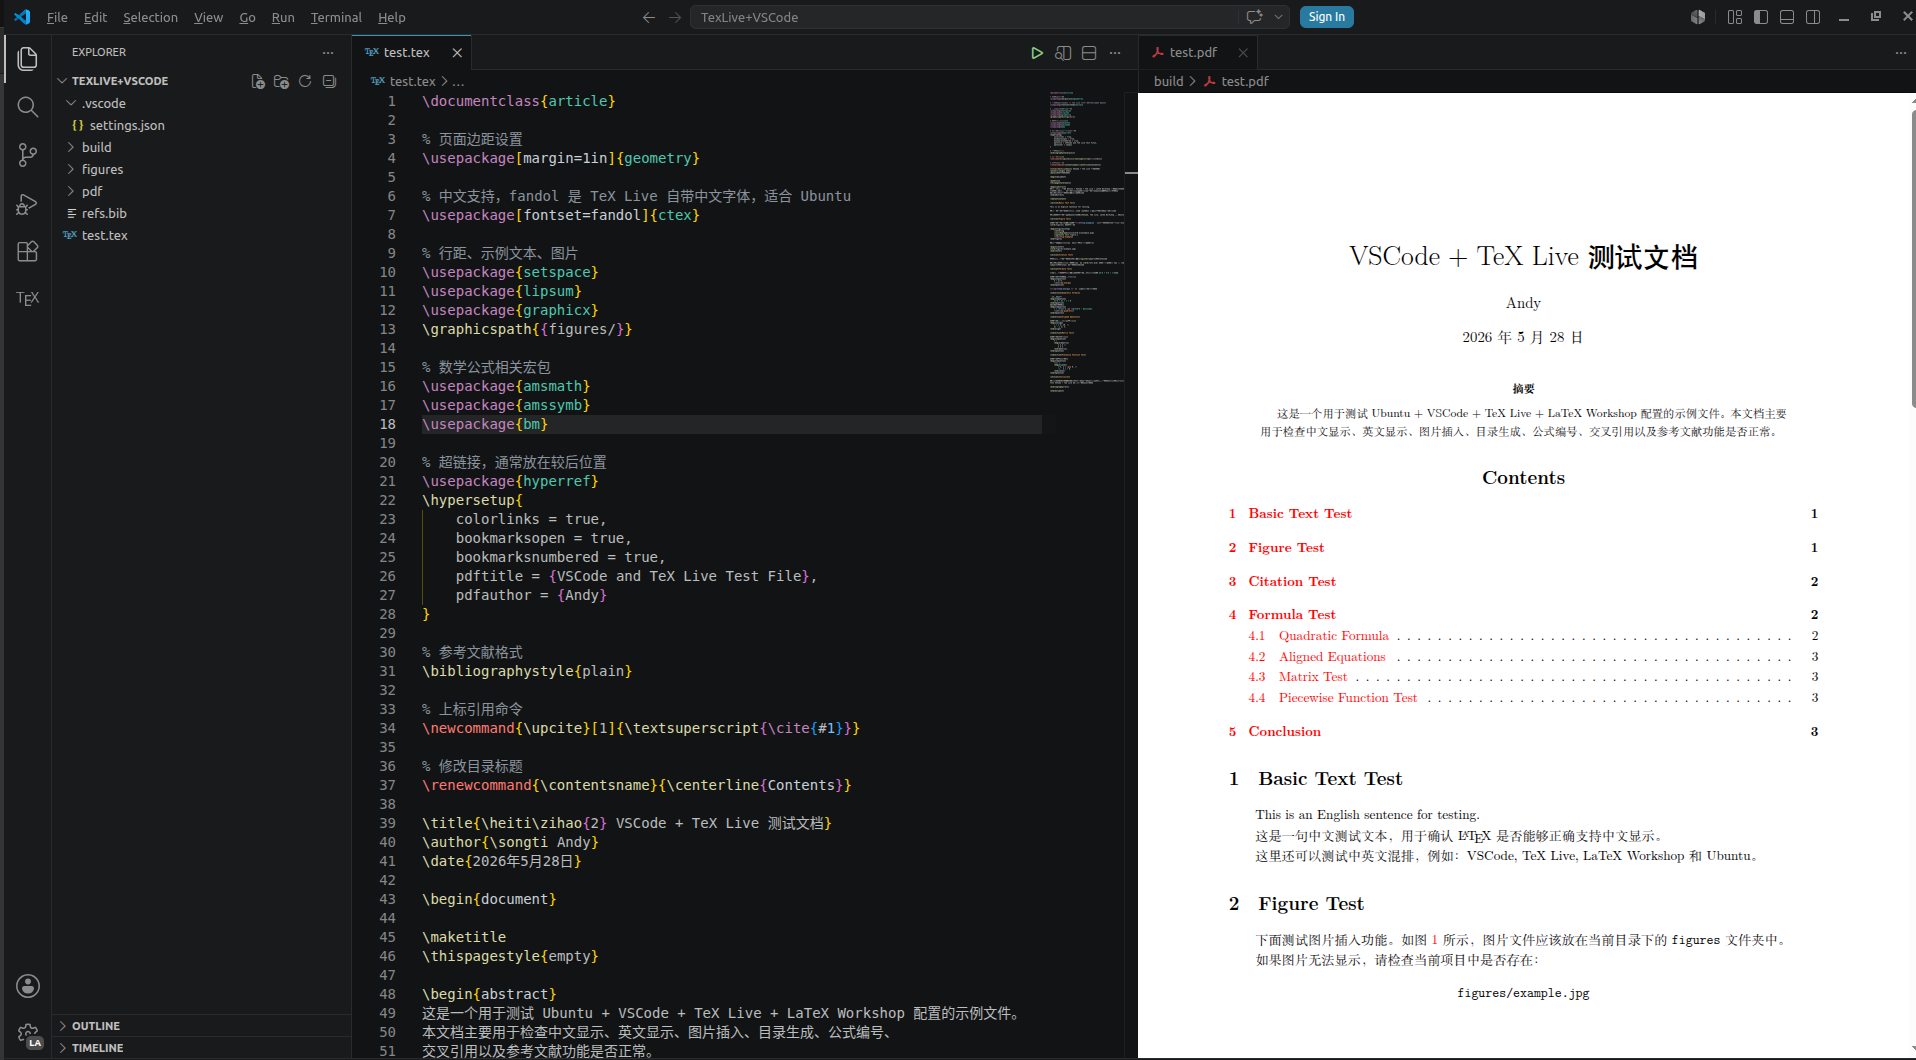
\includegraphics[scale=0.2]{example.png}
	\caption{A test figure.}
	\label{fig:example}
\end{figure}

如果图片无法显示，请检查当前项目中是否存在：

\begin{center}
\verb|figures/example.jpg|
\end{center}

\section{Citation Test}

这句话用于测试参考文献引用功能\upcite{lamport1994latex}。

如果这里的引用显示为问号，请检查 \verb|refs.bib| 文件中是否存在 key 为 \verb|lamport1994latex| 的参考文献条目。

\section{Formula Test}

本节用于测试数学公式功能。首先测试行内公式，例如 $a^2 + b^2 = c^2$。

下面测试带编号的独立公式：
\begin{equation}
	E = mc^2 .
	\label{eq:energy}
\end{equation}

式~\eqref{eq:energy} 是一个简单的公式引用测试。

\subsection{Quadratic Formula}

一元二次方程
\begin{equation}
	ax^2 + bx + c = 0
\end{equation}
的解可以写成：
\begin{equation}
	x = \frac{-b \pm \sqrt{b^2 - 4ac}}{2a}.
	\label{eq:quadratic}
\end{equation}

\subsection{Aligned Equations}

下面测试多行公式对齐环境：
\begin{align}
	x + y &= 10, \\
	2x - y &= 3.
\end{align}

\subsection{Matrix Test}

下面测试矩阵显示：
\begin{equation}
	A =
	\begin{bmatrix}
		1 & 2 \\
		3 & 4
	\end{bmatrix}.
\end{equation}

\subsection{Piecewise Function Test}

下面测试分段函数：
\begin{equation}
	f(x) =
	\begin{cases}
		x^2, & x \geq 0, \\
		-x,  & x < 0.
	\end{cases}
\end{equation}

\section{Conclusion}

如果本文档可以成功编译，并且中文、图片、公式、引用和参考文献都能正常显示，
说明 VSCode + TeX Live 的基本配置已经完成。

\bibliography{refs}

\end{document}

